%%% LaTeX Template: Two column article
%%%
%%% Source: http://www.howtotex.com/
%%% Feel free to distribute this template, but please keep to referal to http://www.howtotex.com/ here.
%%% Date: February 2011

%%% Preamble
\documentclass[	DIV=calc,%
							paper=a4,%
							fontsize=12pt,%
							onecolumn]{scrartcl}	 					% KOMA-article class

\usepackage{lipsum}			% Package to create dummy text
\usepackage[brazil]{babel}	% English language/hyphenation
\usepackage[protrusion=true,expansion=true]{microtype}	% Better typography
\usepackage{amsmath,amsfonts,amsthm}					% Math packages
\usepackage[pdftex]{graphicx}							% Enable pdflatex
\usepackage[svgnames]{xcolor}			% Enabling colors by their 'svgnames'
\usepackage[hang, small,labelfont=bf,up,textfont=it,up]{caption}	% Custom captions under/above floats
\usepackage{epstopdf}						% Converts .eps to .pdf
\usepackage{subfig}							% Subfigures
\usepackage{booktabs}		% Nicer tables
\usepackage{float}

\usepackage{fix-cm}													% Custom fontsizes
\usepackage[utf8]{inputenc}
\usepackage[top=2.5cm, bottom=2.5cm, left=2.5cm, right=2.5cm]{geometry}
\usepackage[ddmmyyyy]{datetime}
\addto\captionsenglish{%
	\renewcommand\tablename{Tabela}
	\renewcommand\figurename{Figura}
} 



%%% Custom sectioning (sectsty package)
\usepackage{sectsty}													% Custom sectioning (see below)
\allsectionsfont{%															% Change font of al section commands
	\usefont{OT1}{phv}{b}{n}%										% bch-b-n: CharterBT-Bold font
}

\sectionfont{%																% Change font of \section command
	\usefont{OT1}{phv}{b}{n}%										% bch-b-n: CharterBT-Bold font
}



%%% Headers and footers
\usepackage{fancyhdr}												% Needed to define custom headers/footers
\pagestyle{fancy}														% Enabling the custom headers/footers
\usepackage{lastpage}
\usepackage{enumitem}
\setlist{nosep}	

% Header (empty)
\lhead{}
\chead{}
\rhead{}
% Footer (you may change this to your own needs)

%% ====================================
%% ====================================
%% mude o rodape  do projeto
%% ====================================
%% ====================================

\lfoot{\footnotesize \texttt{Cabeamento estruturado} \textbullet ~Projeto}


\cfoot{}
\rfoot{\footnotesize página \thepage\ de \pageref{LastPage}}	% "Page 1 of 2"
\renewcommand{\headrulewidth}{0.0pt}
\renewcommand{\footrulewidth}{0.4pt}



%%% Creating an initial of the very first character of the content
\usepackage{lettrine}
\newcommand{\initial}[1]{%
     \lettrine[lines=3,lhang=0.3,nindent=0em]{
     				\color{DarkGoldenrod}
     				{\textsf{#1}}}{}}



%%% Title, author and date metadata
\usepackage{titling}															% For custom titles

\newcommand{\HorRule}{\color{DarkGoldenrod}%			% Creating a horizontal rule
									  	\rule{\linewidth}{1pt}%
										}

\pretitle{\vspace{-30pt} \begin{flushleft} \HorRule 
				\fontsize{50}{50} \usefont{OT1}{phv}{b}{n} \color{DarkRed} \selectfont 
				}

%% ====================================
%% ====================================
%% mude o titulo  do projeto
%% ====================================
%% ====================================

\title{Infraestrutura de Rede para Escritório e Armazém de Produtos}					% Title of your article goes here

%% ====================================



\posttitle{\par\end{flushleft}\vskip 0.5em}

\preauthor{\begin{flushleft}
					\large \lineskip 0.5em \usefont{OT1}{phv}{b}{sl} \color{DarkRed}}
\author{Carlos Alberto Zanella e Danilo Mendes Pusch}  	% Author name goes here


\postauthor{\footnotesize \usefont{OT1}{phv}{m}{sl} \color{Black} 
					\\Universidade Tecnológica Federal do Paraná - Câmpus Cornélio Procópio 								% Institution of author
					\par\end{flushleft}\HorRule}

\date{}																				% No date




%%% Begin document
\begin{document}
\maketitle
\thispagestyle{fancy} 	
\thispagestyle{empty}		% Enabling the custom headers/footers for the first page 
% The first character should be within \initial{}




%% ====================================
%% ====================================
%% mude o resumo  do projeto
%% ====================================
%% ====================================

\initial{E}\textbf{ste projeto irá prover uma infraestrutura de rede de dados para atender a demanda necessária de rede cabeada para um escritório administrativo e um armazém de produtos. As premissas deste projeto são uma rede cabeada projetada de alta velocidade (até 10 Gigabit), onde cada ponto de rede permita a instalação de no mínimo 2 dispositivos de rede por local de trabalho (por exemplo computador e telefone). Deverá contemplar também pontos de rede no escritório para a instalação de dispositivos de rede sem fio. Entre as etapas desse projeto estão contemplados o levantamento da planta física, elaboração da planta lógica, memorial descritivo dos equipamentos passivos de rede, o levantamento da quantidade / custos, o plano de certificação e o orçamento.  \ref{fig4}.}


%% ====================================
\begin{figure}
	\centering
	
\includegraphics{utfpr}
\end{figure}

\vspace{2cm}
\centerline{\textit{\textbf{\today}}}

\clearpage
    \renewcommand*\listfigurename{Lista de figuras}
\listoffigures

\renewcommand*\listtablename{Lista de tabelas}
\listoftables




\clearpage
\renewcommand{\contentsname}{Sumário}
\tableofcontents
\clearpage

%% ====================================
%% ====================================
%% Inicio do texto
%% ====================================
%% ====================================
\section{Introdução}
Este projeto visa implementar infraestrutura de rede com cabeamento estruturado para um novo escritório administrativo e um novo armazém de produtos na Gerência de Manutenção Operacional de uma grande cooperativa agroindustrial. Apesar do projeto ser real, a identidade e o porte do cliente serão omitidos por motivo de confidencialidade. 

\subsection{Benefícios}
A implementação desse projeto deve trazer como benefícios primeiramente facilitar o gerenciamento e garantir a segurança da rede tanto para o escritório administrativo como para o armazém de insumos. Além disso deve contemplar a possibilidade de uma possível expansão futura e atender a requisitos baseados em normas técnicas, além de fornecer a performance necessária para a execução de todas as aplicações.

\subsection{Organizações Envolvidas}
Este projeto, apesar de ser real, por motivo de confidencialidade não identificaremos a organização envolvida. Todo projeto será executado por equipe própria, não envolvendo outras empresas na execução, exceto na aquisição de equipamentos e instalação dos troncos de telefonia. Os perfis de funcionários envolvidos são:
\begin{itemize}
	\item Analista de compras: realizar cotação e compra dos equipamentos. 
	\item Analista financeiro: responsável pela aprovação financeira e pagamentos.
	\item Engenheiro elétrico: realiza o acompanhamento das instalações elétricas necessárias. 
	\item Desenhista: realiza as plantas físicas e lógicas do projeto. 
	\item Instalador: responsável por realizar a instalação dos passivos de rede conforme projeto. 
	\item Analista de TI: acompanha e ativa a conectividade de acesso a rede da empresa. 
	\item Empresa de telecom: instala os troncos de telefonia.  
\end{itemize}


\section{Estado atual}
Como os ambientes em que o projeto será implementado são novos e acabam de ser construídos, o estado atual da rede não se aplica a essa situação. 

\section{Requisitos}
Provisionar uma rede cabeada projetada de alta velocidade (até 10 Gigabit). Permitir a instalação de no mínimo 2 dispositivos de rede por local de trabalho (telefone IP / micro ou Thin Client). Pontos de rede adicionais para instalação de dispositivos sem fio (Wi-Fi) e também para possível expansão posterior. 

\section{Usuários e Aplicativos}
Este ambiente deverá comportar uma central de distribuição da empresa. A principio a quantidade de usuários nesse setor deverá ser a que consta na relação abaixo, sem uma previsão inicial de expansão. O projeto deve permitir a instalação de equipamentos para rede sem-fio (Wi-Fi) com pontos de rede já devidamente previstos e instalados. 


\subsection{Usuários}
A central de distribuição deverá contar com a seguinte equipe:
\\
\begin{itemize}

	\item 6 auxiliares administrativos;
	\item 2 faturistas;
	\item 1 secretária;
	\item 4 estoquistas;
	\item 2 analistas de RH;
	\item 1 chefe de departamento.
		
\end{itemize}

\subsection{Aplicativos}
Relação dos aplicativos e seus níveis críticos de uso.
\\
\begin{itemize}

	\item ERP (Uniface): criticidade alta. 
	\item Sistema de gestão de ativos (IBM Maximo): criticidade média.
	\item Sistema dos coletores: criticidade média. 
	\item Arterisk telefonia IP: criticidade alta. 
	\item Sistema operacional Windows: criticidade média.  
	\item Pacote Office: criticidade média. 
\end{itemize}


\section{Estrutura predial existente}
Estrutura predial existente conforme figura \ref{figura1}. 

%INTERVENÇÃO - DBARROS # 

\subsection{Topologia}
De acordo com Augusto \cite{ID1}, a topologia pode ser entendida como a maneira pela qual os enlaces de comunicação e dispositivos de comutação estão interligados, provendo efetivamente a transmissão do sinal entre nós da rede. [...] Podemos dizer que a topologia física de uma rede local compreende os enlaces físicos de ligação dos elementos computacionais da rede, enquanto a topologia lógica da rede se refere à forma através da qual o sinal é efetivamente transmitido entre um computador e outro. A topologia implementada para este ambiente é a topologia em árvore. Respectivamente, temos a planta baixa conforme figura \ref{figura2}, a planta lógica conforme a figura \ref{figura3}.



%inicio dos comandos para criar uma nova pagina A3 horizontal
\clearpage
\thispagestyle{plain}
\KOMAoptions{paper=a3, paper=landscape, DIV=20}

\recalctypearea
%\subsection{Planta Física Cabeada}

\begin{figure}
	%	\centering
	\noindent\makebox[\textwidth][c]{
		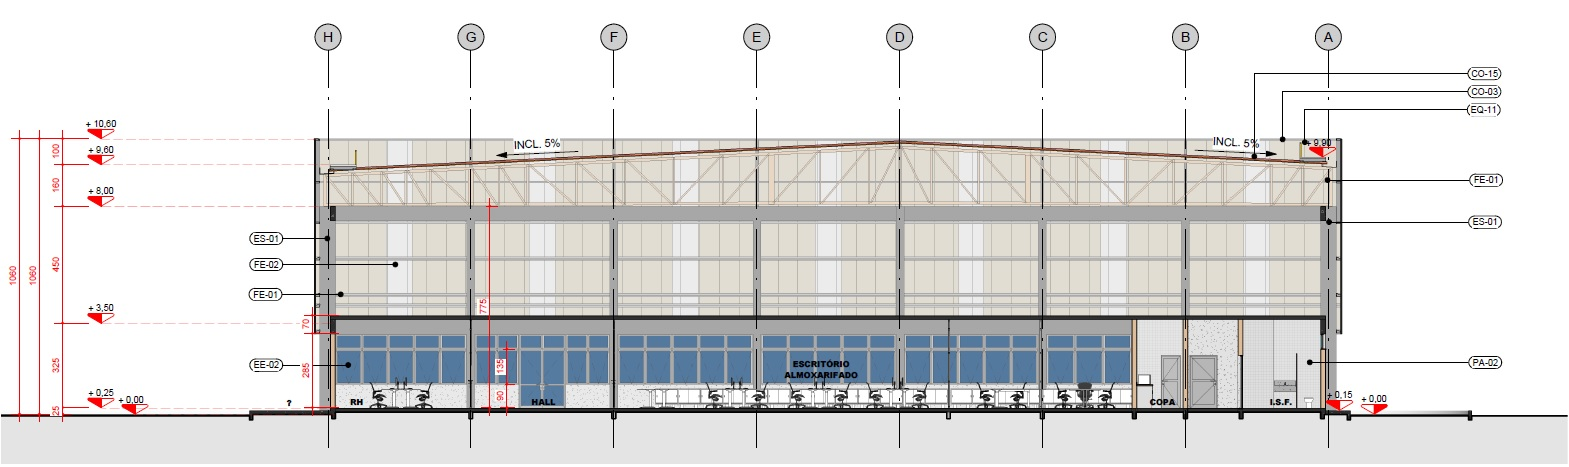
\includegraphics[width=\textwidth]{figura1}
	}
	\caption{Estrutura predial existente - Formato A3.}
	\label{figura1}
\end{figure}

%Retornar ao formato A4
\clearpage
\KOMAoptions{paper=a4, paper=portrait, DIV=15}
\recalctypearea
%-- reinicio em A4 



%%%%%%%%%%%%%%%%%%%%% ANTIGO %%%%%%%%%%%%%%%%%%%%%%%%
%\begin{figure}
	%\centering
	%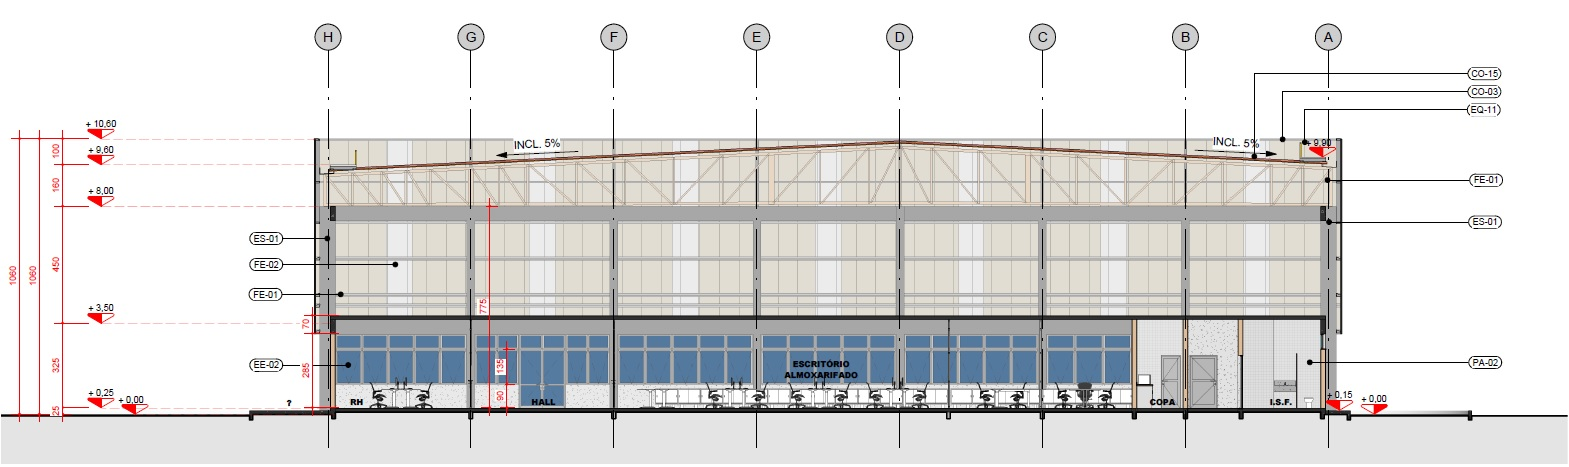
\includegraphics[width=\textwidth]{figura1}
	%\caption{Estrutura predial existente}
	%\label{figura1}
%\end{figure}




%INTERVENÇÃO - DBARROS # 2

%inicio dos comandos para criar uma nova pagina A3 horizontal
\clearpage
\thispagestyle{plain}
\KOMAoptions{paper=a3, paper=landscape, DIV=20}

\recalctypearea
%\subsection{Planta Física Cabeada}

\begin{figure}
	%	\centering
	\noindent\makebox[\textwidth][c]{
		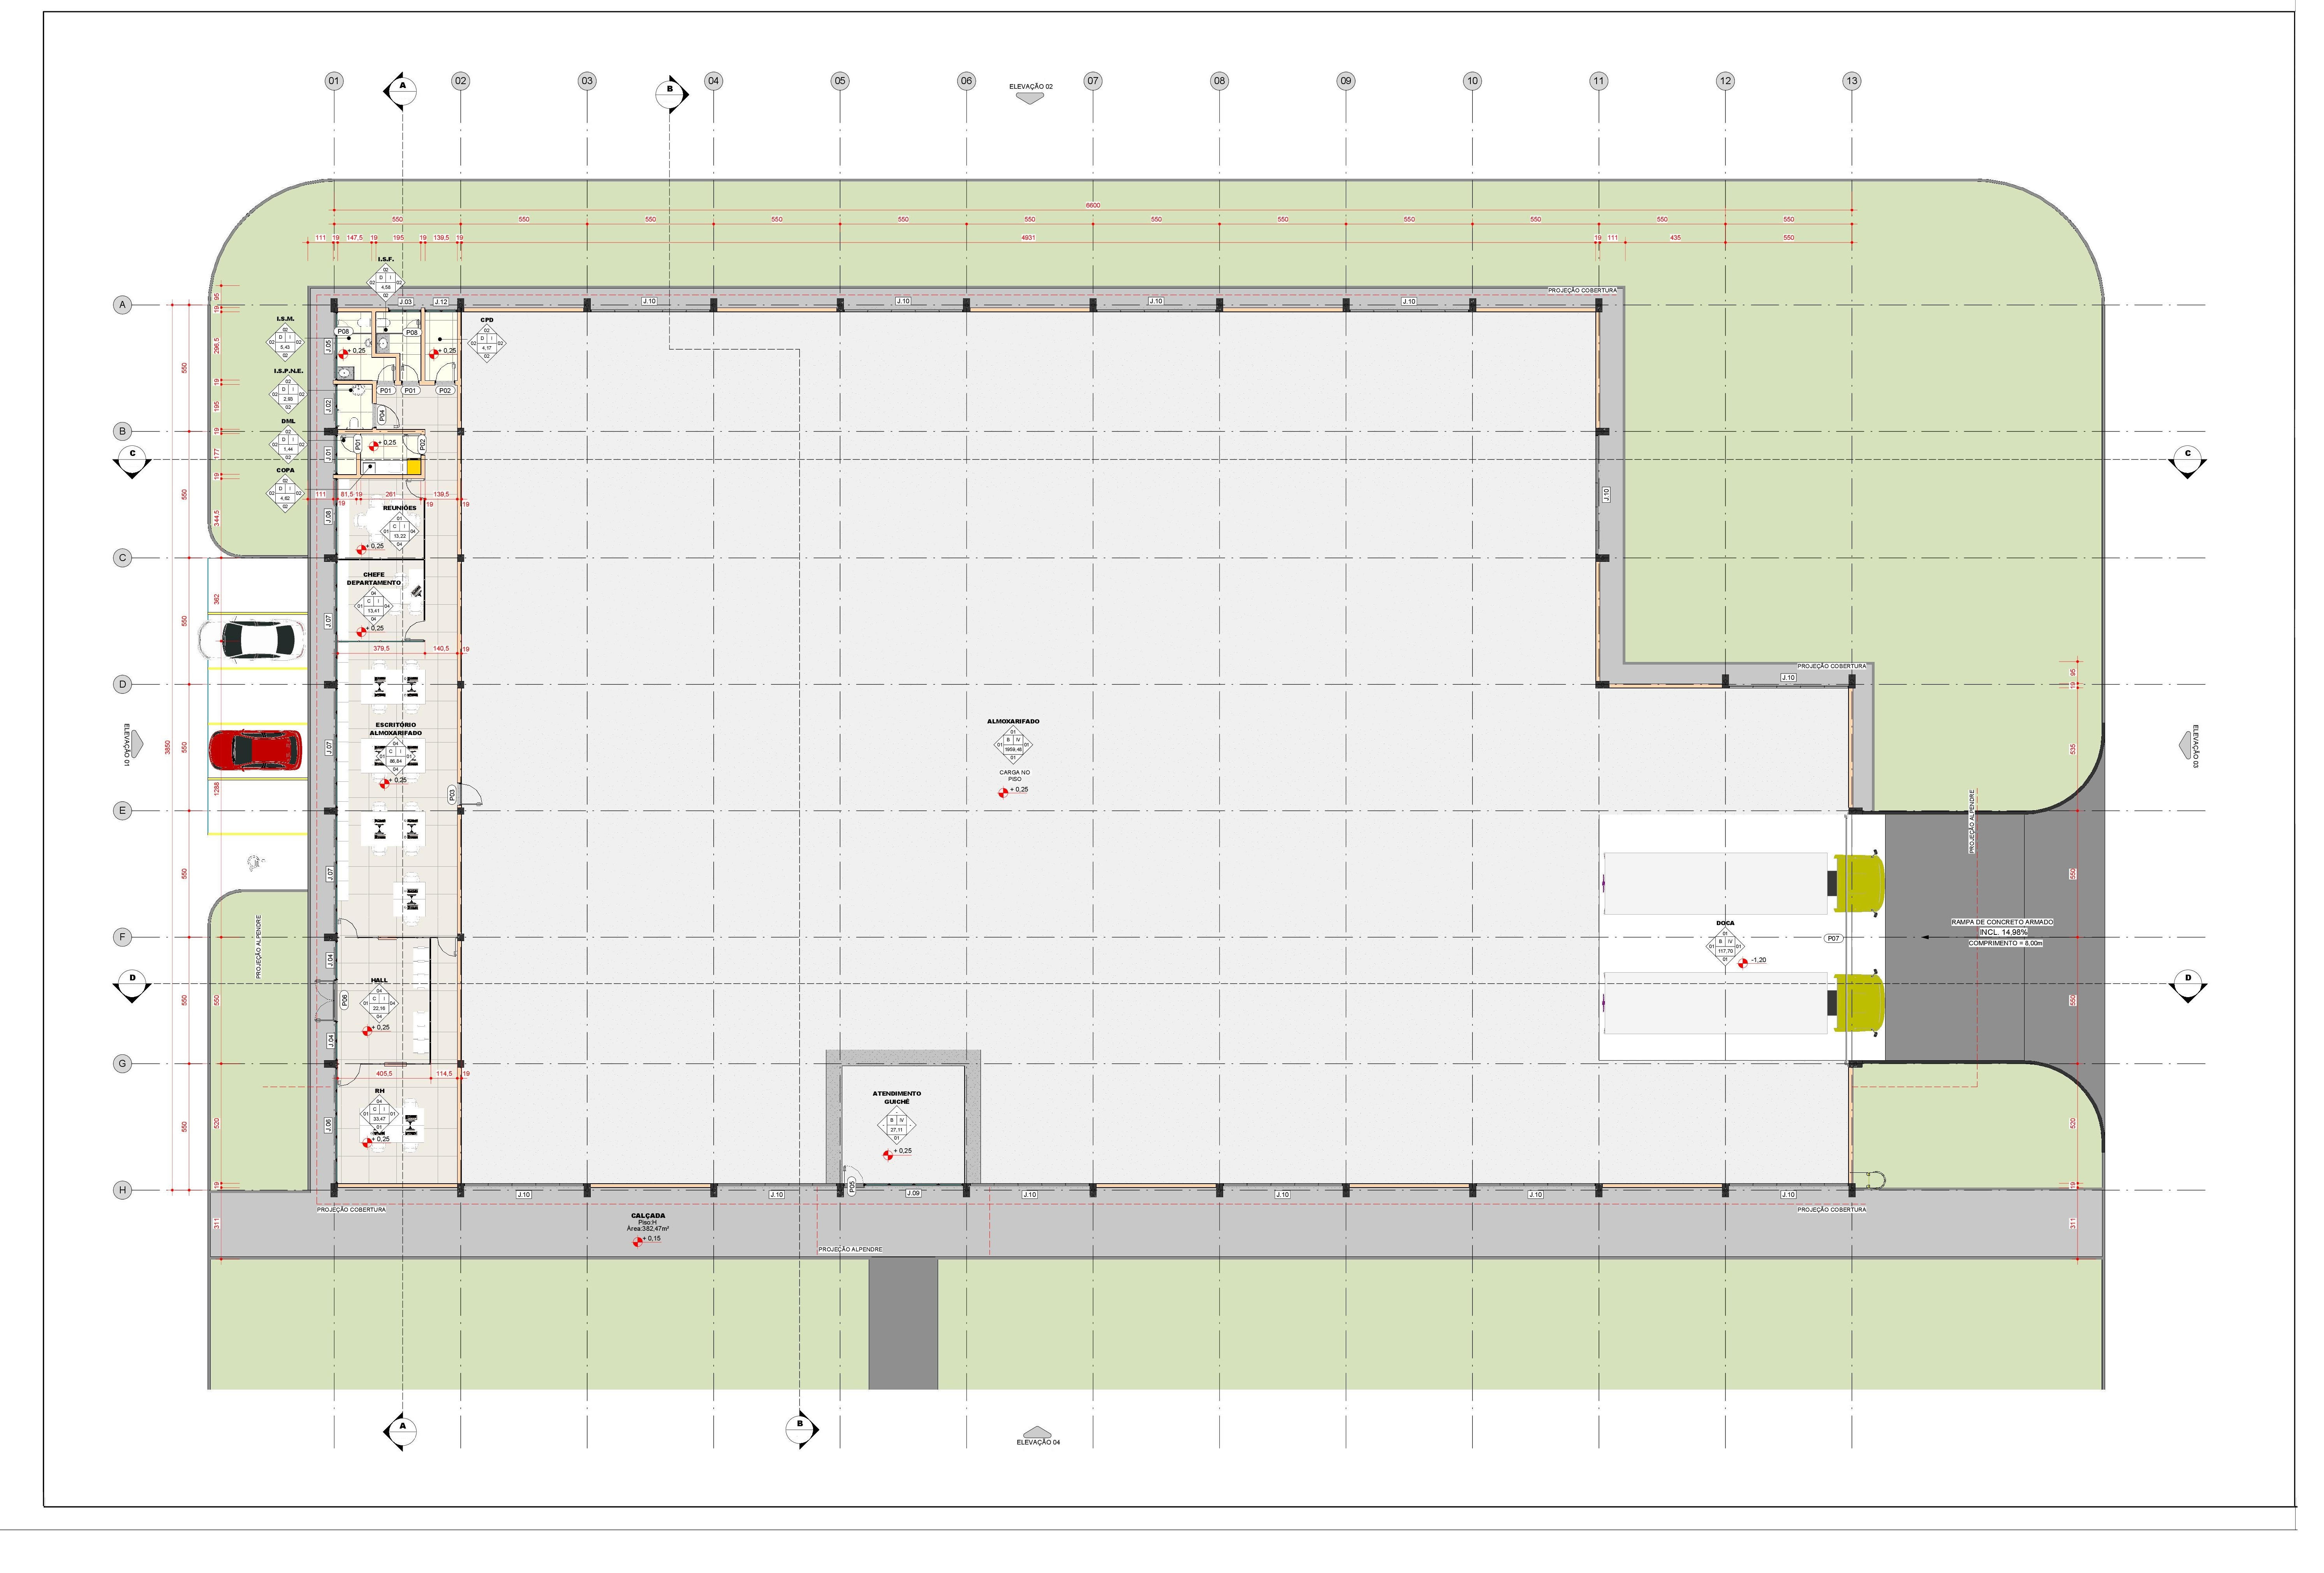
\includegraphics[width=\textwidth]{figura2}
	}
	\caption{Planta Baixa - Formato A3.}
	\label{figura2}
\end{figure}

%Retornar ao formato A4
\clearpage
\KOMAoptions{paper=a4, paper=portrait, DIV=15}
\recalctypearea
%-- reinicio em A4 



%%%%%%%%%%%%%%%%%%%%% ANTIGO %%%%%%%%%%%%%%%%%%%%%%%%
%\section{Planta Lógica - Elementos estruturados}

%\subsection{Estado atual}
%Planta baixa e situação atual do prédio conforme figura \ref{figura2}. 
%\begin{figure}
	%\centering
	%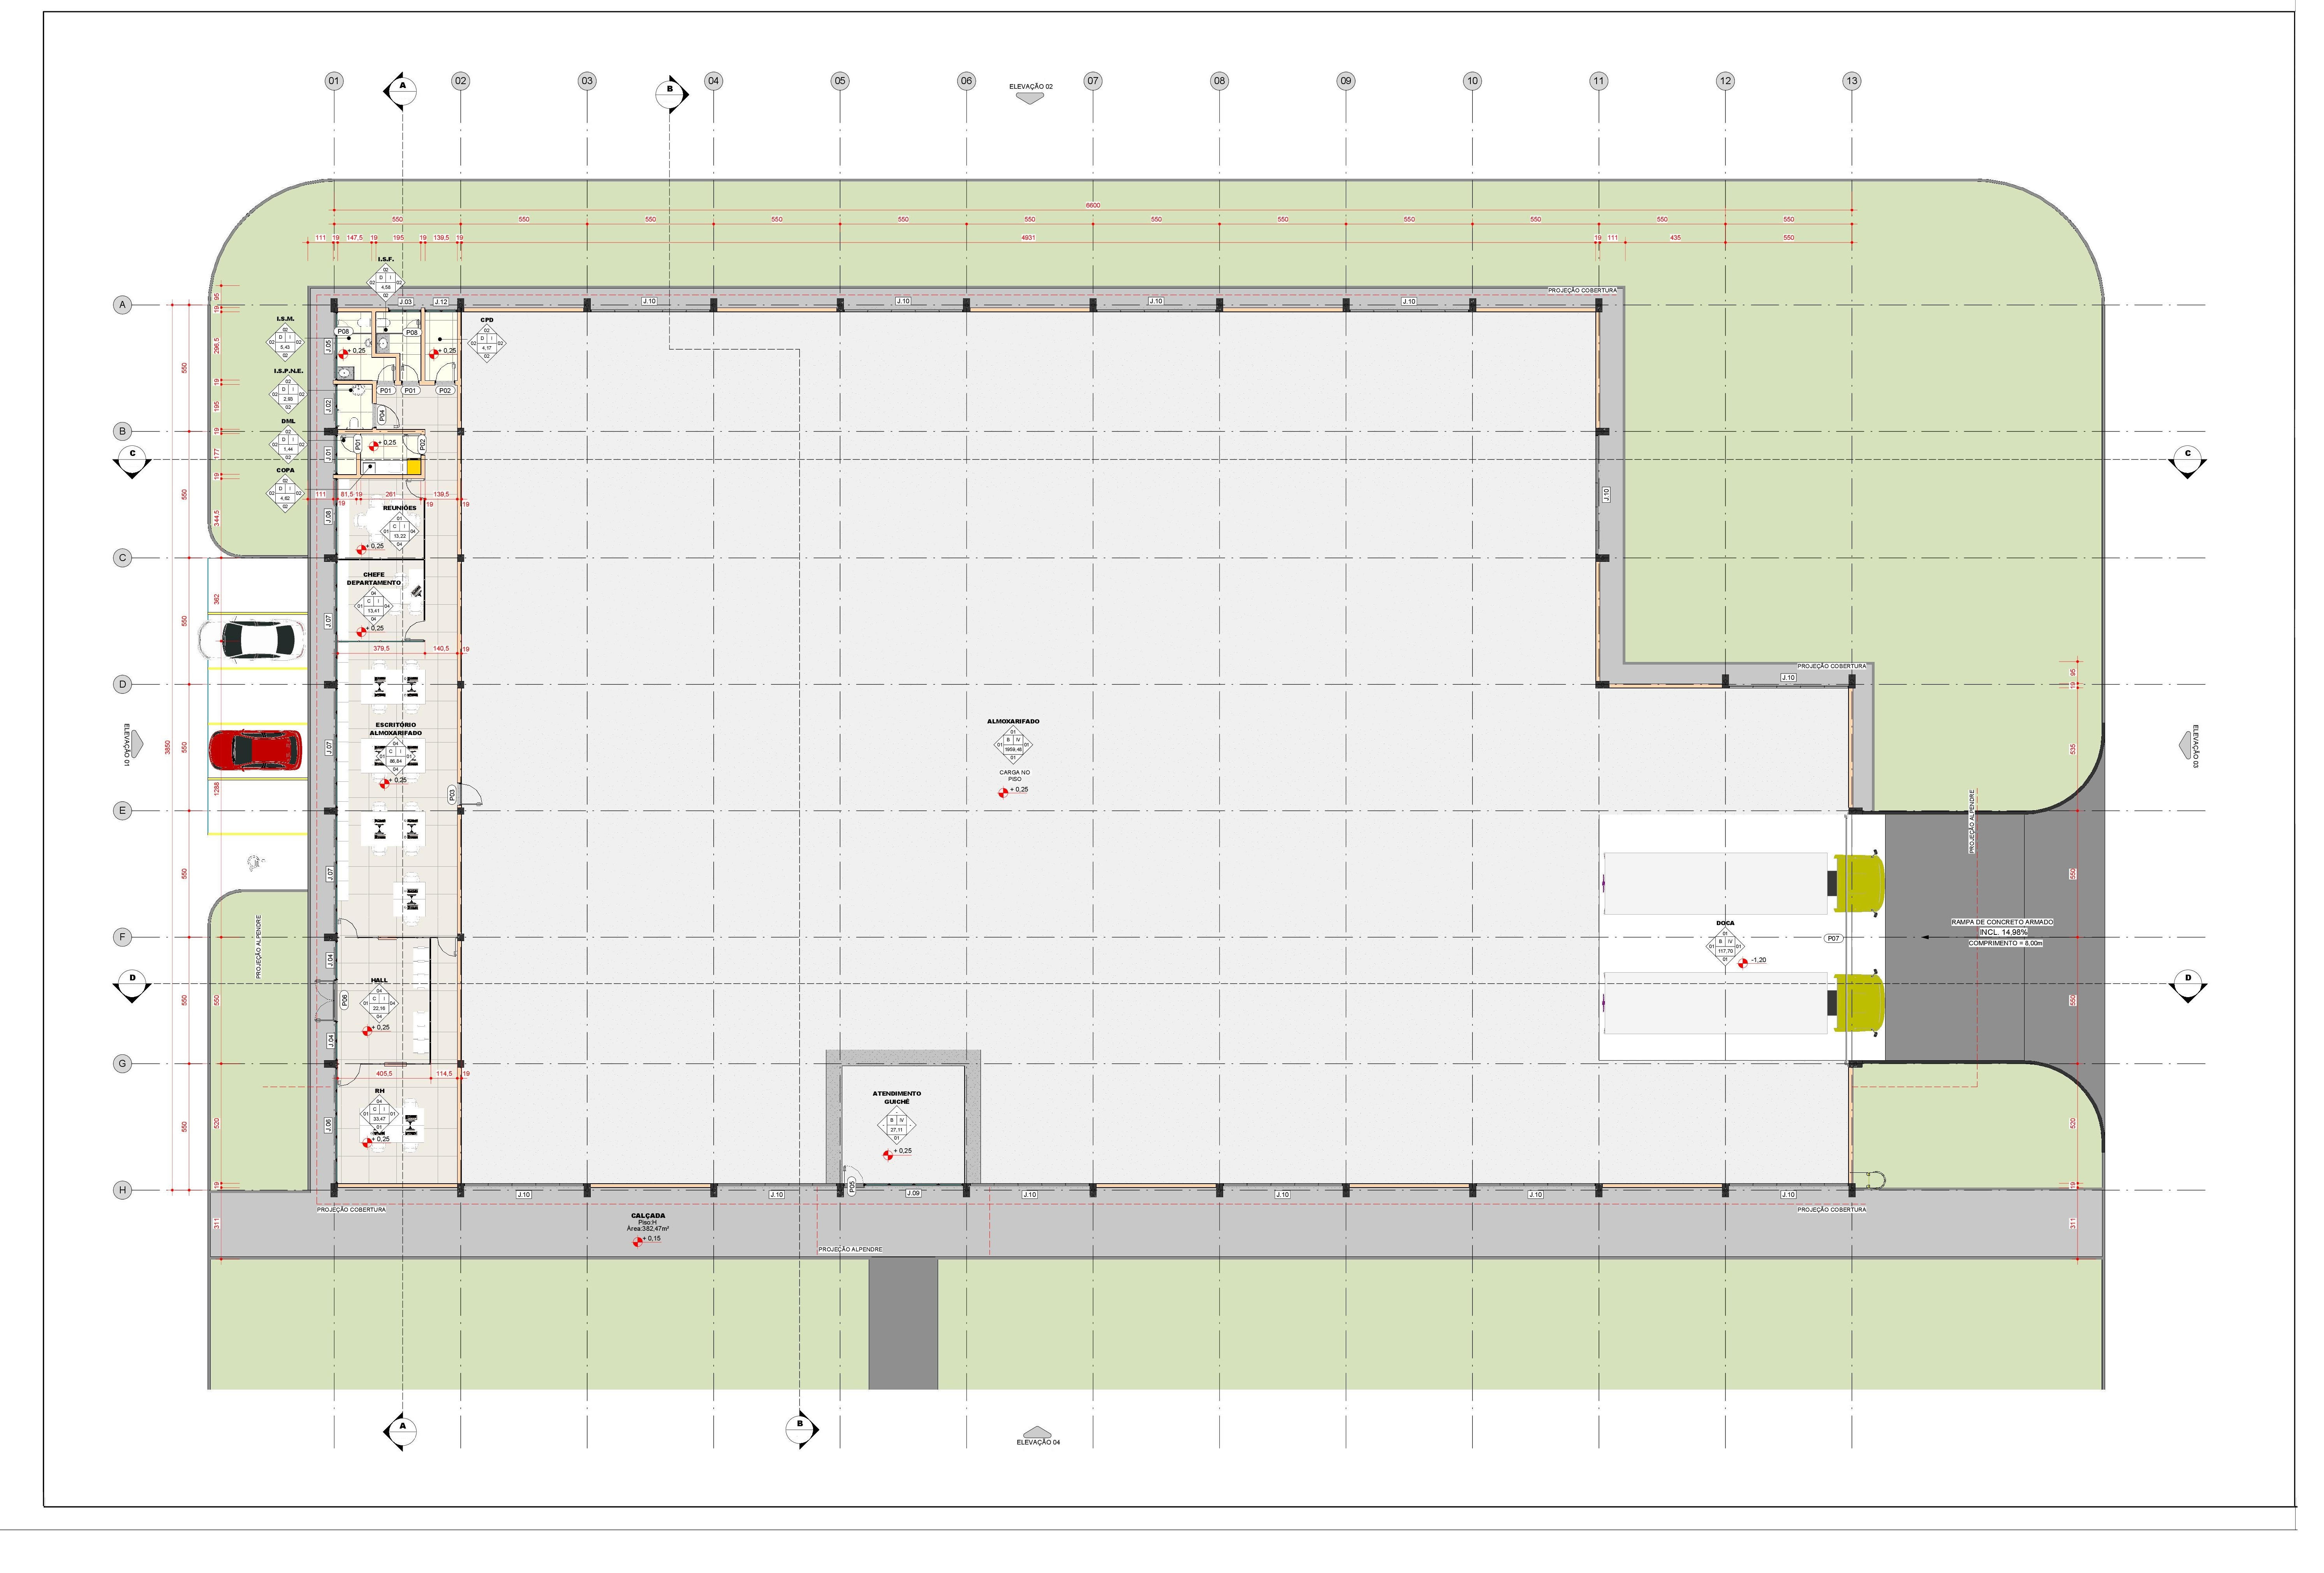
\includegraphics[width=\textwidth]{figura2}
	%\caption{Planta baixa}
	%\label{figura2}
%\end{figure}




%INTERVENÇÃO - DBARROS # 3

%inicio dos comandos para criar uma nova pagina A3 horizontal
\clearpage
\thispagestyle{plain}
\KOMAoptions{paper=a3, paper=landscape, DIV=20}

\recalctypearea
%\subsection{Planta Física Cabeada}

\begin{figure}
	%	\centering
	\noindent\makebox[\textwidth][c]{
		\includegraphics[width=\textwidth]{figura3}
	}
	\caption{Planta Lógica - Formato A3.}
	\label{figura3}
\end{figure}

%Retornar ao formato A4
\clearpage
\KOMAoptions{paper=a4, paper=portrait, DIV=15}
\recalctypearea
%-- reinicio em A4 


%%%%%%%%%%%%%%%%%%%%% ANTIGO %%%%%%%%%%%%%%%%%%%%%%%%
%\begin{figure}
%\centering
%\includegraphics[width=\textwidth]{figura3}
%\caption{Planta lógica}
%\label{figura3}
%\end{figure}


Podemos ver também os modelos de rack que serão utilizados abaixo na tabela \ref{tab1}.

\begin{table}[h!]
\centering
\caption{Exemplo de racks utilizados}
\label{tab1}
\begin{tabular}{|l|l|l|}
\hline
\multicolumn{3}{|l|}{Racks utilizados} \\ \hline
1        & Rack 12U          & 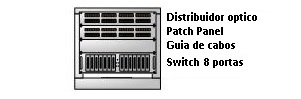
\includegraphics[scale=0.8]{figura5}        \\ \hline
2        & Rack 40U        & 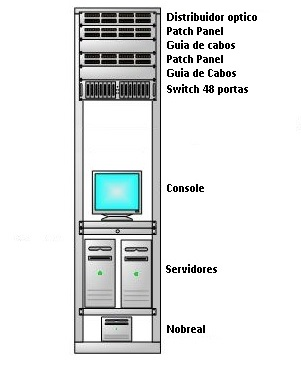
\includegraphics[scale=0.8]{figura6}        \\ \hline
\end{tabular}
\end{table}

\subsection{Encaminhamento}

Relação do encaminhamento e seus respectivos custos conforme figura \ref{figura4}.  
\begin{figure}[H]
	\centering
	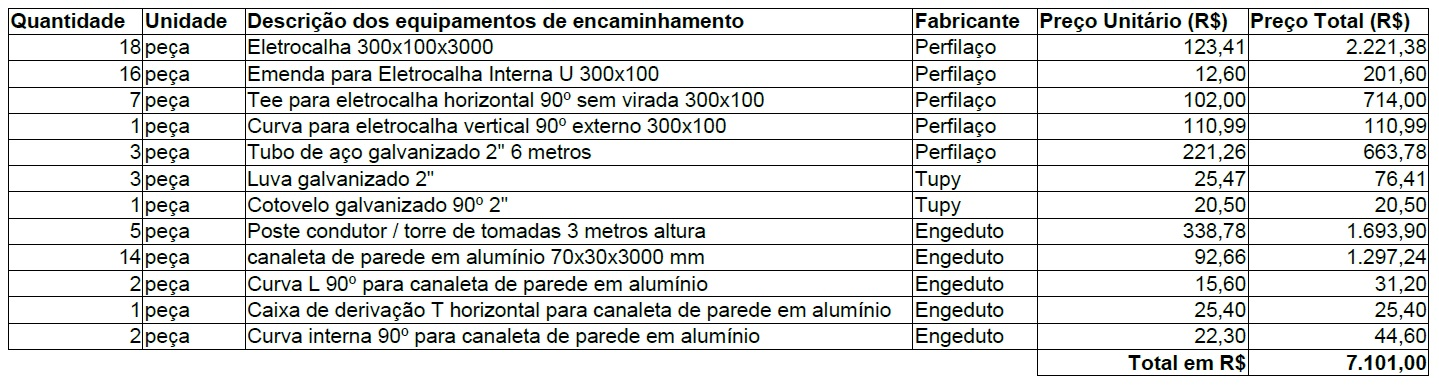
\includegraphics[width=\textwidth]{figura4}
	\caption{Encaminhamento e custos}
	\label{figura4}
\end{figure}

 
\subsection{Memorial descritivo}
Memorial descritivo conforme figura \ref{figura7}.  
\begin{figure}[H]
	\centering
	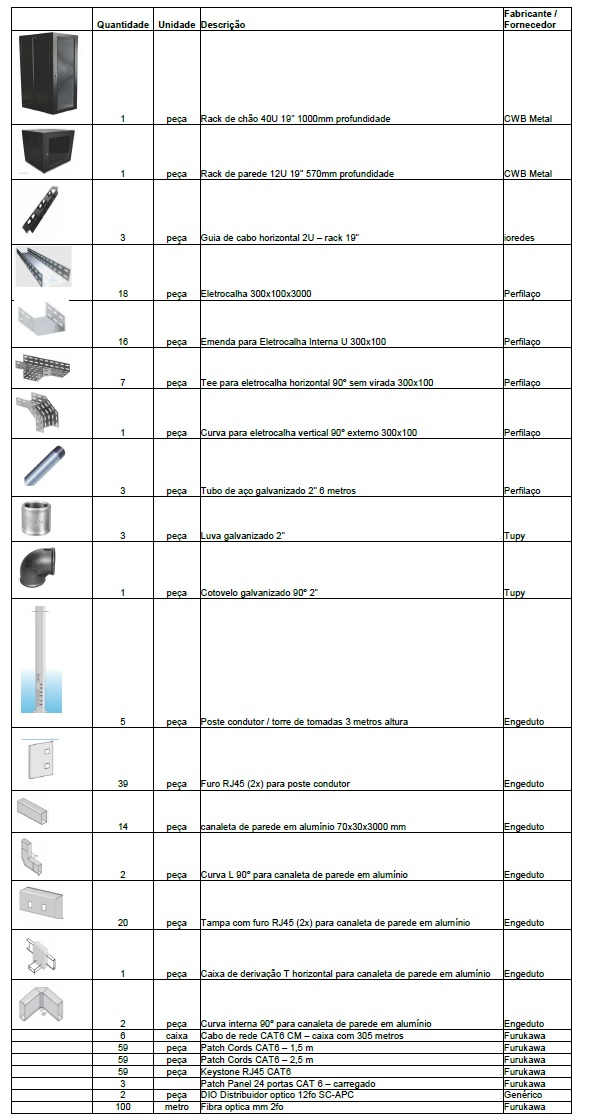
\includegraphics[width=\textwidth,height=24cm]{figura7}
	\caption{Memorial descritivo}
	\label{figura7}
\end{figure}

Relação todos os equipamentos passivos que serão utilizados, tipo, fabricante, quantidade e seus respectivos custos conforme figura \ref{figura8}.  
\begin{figure}[H]
	\centering
	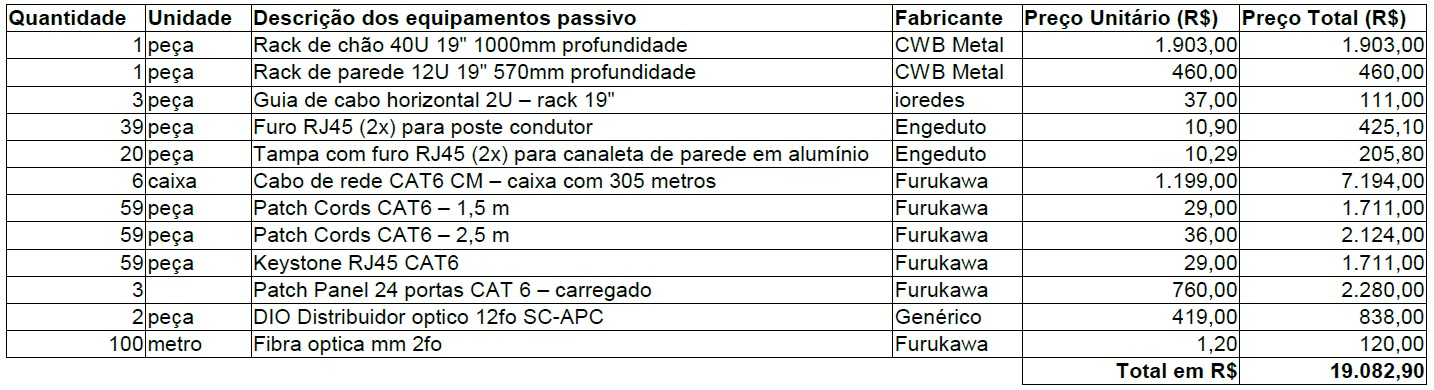
\includegraphics[width=\textwidth]{figura8}
	\caption{Passivos, quantidades e custos}
	\label{figura8}
\end{figure}



\subsection{Identificação dos cabos}
A identificação dos cabos será realizada de acordo com a norma NBR 14565:2000. A relação de todos os passivos utilizados, inclusive os cabos, bem como os custos envolvidos consta no item 6.4, memorial descritivo deste documento. 

\section{Implantação}
Cronograma de implantação conforme figura \ref{cronograma}:

\begin{figure}[h]
	\centering
	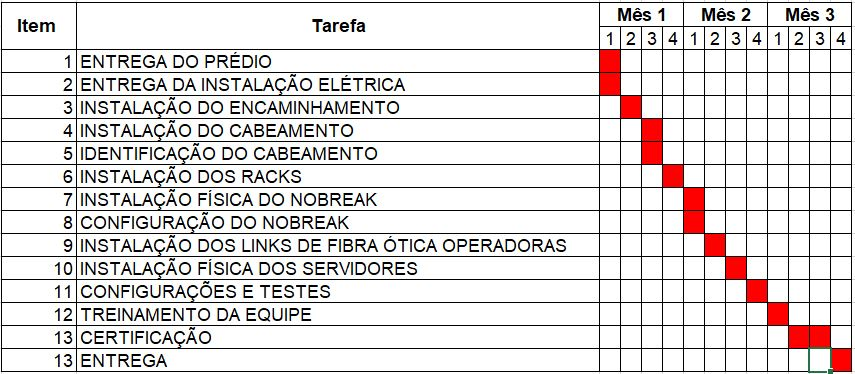
\includegraphics[width=\textwidth]{cronograma}
	\caption{Resumo gráfico}
	\label{cronograma}	
\end{figure}:


\section{Plano de certificação}

A certificação da rede será realizada por empresa terceirizada a ser contratada após sua conclusão física, antes da entrega para uso, em todos os pontos de redes. Será exigido apenas os testes passivos da rede, conhecidos também como testes de campo. Para a rede de pares metálicos, baseado na documentação técnica dos fabricantes,  será exigido os seguintes testes:
\begin{itemize}	
	\item Wiremap;
	\item Lenght;
	\item Attenuation ou Insertion Loss;
	\item NEXT loss (Near and Crosstalk);
	\item OS-NEXT Loss (Power Sum NEXT);
	\item FEXT (Far End Crosstalk);
	\item ELFEXT Loss (Power Sum Equal Far End Crosstalk);
	\item Return Loss;
	\item Propagation Delay;
	\item Delay Skew ou Propagation Delay Skew;
	\item ACR (Atenuation to Crosstalk Ratio);
	\item PS-ACR (Power Sum Attenuation to Crosstalk Ratio);
	\item Alien Crosstalk;
	\item Insertion Loss Deviation;
	\item DCLoop Resistance;	
\end{itemize}

Para a rede de fibra óptica, baseado nas especificações técnica do fabricante, será exigido os seguintes testes:
\begin{itemize}	
	\item Atenuação (Attenuation or Insertion Loss);
	\item Atenuação por retroespelhamento;
	\item Atenuação de inserção;
	\item Teste de comprimento;
\end{itemize}

A empresa contratada deverá fornecer os relatórios de todos testes realizados e um parecer técnico da viabilidade da rede para atender a demanda solicitada, que neste caso seria uma rede de alta velocidade no padrão 10GBASE-T. Fonte: \cite{ID2}, \cite{ID3}


\section{Plano de manutenção}

A manutenção desta rede deverá seguir as melhores práticas e deverá ser registrada no sistema de gestão de Ativos IBM Maximo de acordo com os seguintes critérios: 
\begin{itemize}
	\item Manutenção Preventiva: Realizada mensalmente na Central de Distribuição pelos técnicos do setor de manutenção de informática, subordinado ao departamento de infraestrutura e suporte de TI. Será executado um plano de trabalho onde é realizada a verificação das conexões e a checagem visual do estado geral dos equipamentos, e também a execução da limpeza adequada. 
	\item Manutenção Corretiva (interna): Realizada pelos analistas departamento de infraestrutura e suporte de TI. Consiste na solução dos problemas detectados na manutenção preventiva ou pela abertura de incidentes no sistema de Service Desk.
	\item Manutenção Corretiva (terceiros): Realizada por empresa de suporte externa. Consiste na solução dos problemas detectados na manutenção preventiva ou corretiva não solucionados internamente ou quando envolvem garantias de equipamentos. Consiste na manutenção e/ou troca de componentes. As manutenções corretivas por terceiros são realizadas por empresas contratadas pelo departamento de compras da empresa, negociadas pelo departamento de gestão de TI e com aprovação técnica do departamento de infraestrutura e suporte de TI.
\end{itemize}

\subsection{Plano de expansão}

A expansão da infraestrutura de tecnologia da central de distribuição deverá ser aprovada pela superintendência administrativa da empresa. Posteriormente, serão definidas as configurações de hardwares e softwares necessárias pelo departamento de infraestrutura e suporte de TI, bem como o projeto de implantação deve ser definido pelo setor de gestão de projetos, subordinado ao departamento de gestão de TI. Poderá ser executado por equipe interna do setor de manutenção de TI ou por empresa contratada. 

\section{Risco}
De acordo com Beal \cite{ID4}, uma das grandes vulnerabilidades de segurança encontradas nas organizações são as pessoas que nelas atuam. O abuso de privilégios de acesso a dados ou instalações podem comprometer a segurança. A necessidade de contratação de serviços de terceiros como prestadores de serviço, fornecedores e consultores pode representar sérias ameaças à segurança da informação, caso não sejam auditadas.
A avaliação dos riscos visa comparar dados coletados anteriormente na análise de riscos com os critérios de risco, considerando a tolerância da organização perante os mesmos. Caso haja necessidade, uma análise mais aprofundada do risco deverá ser empregada a norma (ABNT NBR ISO/IEC 31000:2009). Ainda segundo Beal \cite{ID4}, a avaliação dos riscos deverá ser efetuada por pessoas qualificadas, que possuam características como:
\begin{itemize}	
	\item Conhecimento dos ativos e sua importância para a organização; 
	\item Formação técnica na área a ser avaliada;
	\item Experiência e conhecimento das práticas, procedimentos e princípios de segurança da informação;
	\item Conhecimento da metodologia e das ferramentas a serem utilizadas na avaliação de riscos. 
\end{itemize}

Tendo isso em vista, o projeto de avaliação de riscos deve ser elaborado por área competente e levar em consideração esses itens que não compreendem exatamente competência da área técnica:
\begin{itemize}	
	\item Atraso na entrega do prédio; 
	\item Atraso na entrega da instalação elétrica;
	\item Atraso na instalação do encaminhamento e do cabeamento; 
	\item Atraso na instalação dos racks e no break; 
	\item Atraso na instalação dos links de fibra ótica pelas operadoras; 
	\item Entre outros riscos técnicos avaliados pela área competente. 
	
\end{itemize}


\section{Orçamento}
O orçamento total para o projeto é de R\$ 26183,90 (Vinte e seis mil, cento e oitenta e três Reais e noventa centavos), conforme detalhado nos itens 5.2 Encaminhamento e 5.3 Memorial descritivo deste documento. 

\section{Recomendações}
É proibida a utilização da infraestrutura de encaminhamento de cabo para a passagem de cabos de energia
elétrica. No entanto, em casos especiais, e com o uso de dutos com separação entre os cabos de energia elétrica e
de comunicação, poderá haver este compartilhamento, que será autorizado após analise pela equipe técnica do
departamento de infraestrutura e suporte de TI. A passagem de outros cabos de sinal (som, alarmes, sinalização, etc) devem ser previamente submetidos ao departamento de infraestrutura e suporte de TI para aprovação, sendo necessário fornecer as especificações técnicas (tensões, correntes, interfaces, meio físico, nível de radiação eletromagnética, etc) do sistema a ser implantado.

\section{Resumo gráfico}

Mapa mental do projeto conforme figura \ref{mapa_mental}:

\begin{figure}[h]
	\centering
	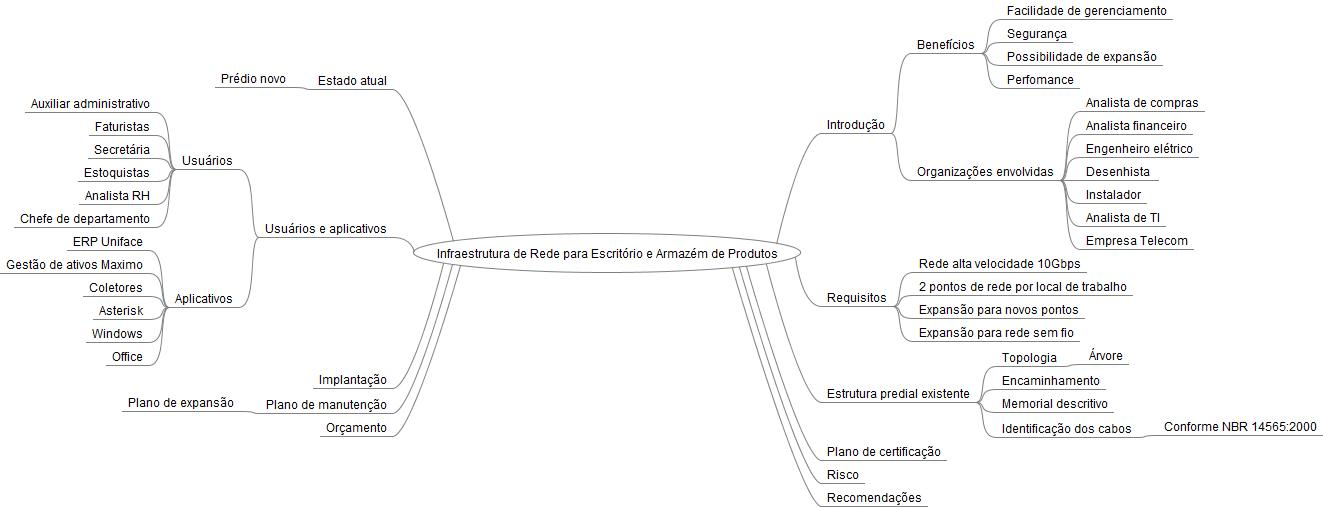
\includegraphics[width=\textwidth,height=10cm,keepaspectratio]{mapa_mental}
	\caption{Resumo gráfico}
	\label{mapa_mental}	
\end{figure}

\section{Referências bibliográficas}

\renewcommand\refname{} %%Referências bibliográficas}  
\bibliographystyle{ieeetr}
\bibliography{referencias}  

\end{document}